\documentclass{ctexart}
\usepackage[T1]{fontenc}
\usepackage[a4paper,top=1.5cm,bottom=1.5cm,left=2cm,right=2cm,marginparwidth=1.75cm]{geometry}
\usepackage{mathtools}
\usepackage{tikz}
\usepackage{booktabs}
\usepackage{caption}
\usepackage{outlines}
\usepackage{graphicx}
\usepackage{float}
\usepackage{amsthm}
\usepackage{tabularray}
\usepackage{minted}
\usepackage[colorlinks=false, allcolors=blue]{hyperref}
\usepackage{cleveref}
\renewcommand{\tableautorefname}{表}
\usetikzlibrary{automata,positioning}
\UseTblrLibrary{booktabs}
\DeclarePairedDelimiter{\set}{\{}{\}}
\DeclarePairedDelimiter{\paren}{(}{)}
\graphicspath{ {./images/} }

\newcounter{fullrefcounter}
\newcommand*{\fullref}[1]{%
\addtocounter{fullrefcounter}{1}%
\label{--ref-\thefullrefcounter}%
\ifthenelse{\equal{\getpagerefnumber{--ref-\thefullrefcounter}}{\getpagerefnumber{#1}}}
  {
    \hyperref[{#1}]{\Cref*{#1} \nameref*{#1}}
  }
  {% false case
    \hyperref[{#1}]{第 \pageref*{#1} 页 \Cref*{#1} \nameref*{#1}}
  }
}

\title{编译原理作业}
\author{卢雨轩 19071125}
% \date{\today}
\ctexset{
    section = {
        titleformat = \raggedright,
        name = {,},
        number = \chinese{section}、
    },
    paragraph = {
        runin = false
    },
    today = small,
    figurename = 图,
    contentsname = 目录,
    tablename = 表,
}

\begin{document}

\maketitle

\begin{outline}
    \1[8.] \2[(3)] (35 - 28) * 8 \\

    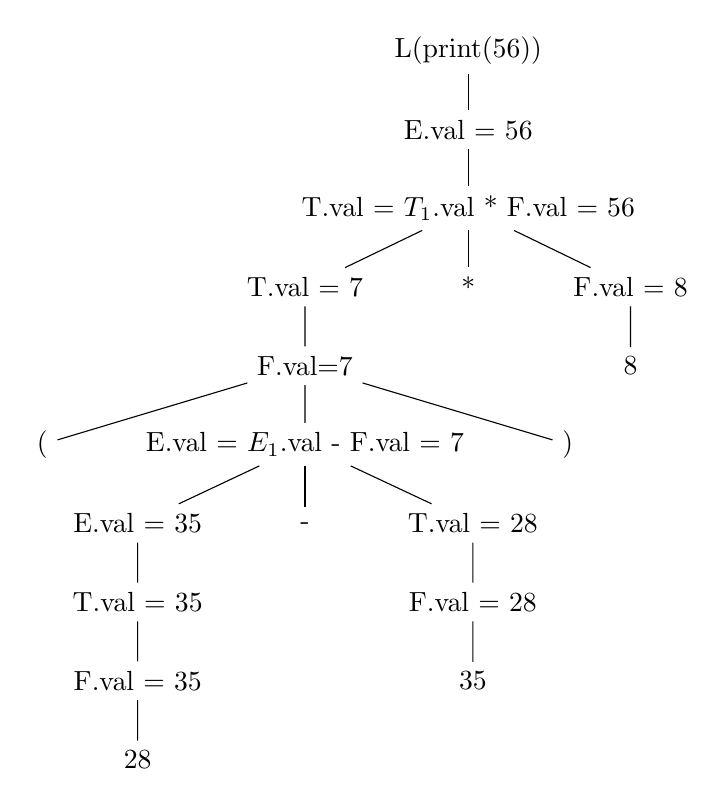
\begin{tikzpicture}
        \node(1) {L(print(56))};
        \node(2)[below of=1] {E.val = 56};
        \node(3)[below of=2] {T.val = $T_1$.val * F.val = 56};
        \node(4)[below of=3] {*};
        \node(5)[left=1cm of 4] {T.val = 7};
        \node(6)[right=1cm of 4] {F.val = 8};
        \node(7)[below of=5] {F.val=7};
        \node(8)[below of=6] {8};
        \node(9)[below of=7] {E.val = $E_1$.val - F.val = 7};
        \node(123)[left=1cm of 9]{(};
        \node(321)[right=1cm of 9]{)};
        \node(10)[below of=9] {-};
        \node(11)[left = 1cm of 10] {E.val = 35};
        \node(12)[right=1cm of 10] {T.val = 28};
        \node(13)[below of=11] {T.val = 35};
        \node(14)[below of=12] {F.val = 28};
        \node(15)[below of=13] {F.val = 35};
        \node(16)[below of=14] {35};
        \node(17)[below of=15] {28};

        \draw (1) -- (2) -- (3) -- (4);
        \draw (3) -- (6) -- (8) ;
        \draw (3) -- (5) -- (7) -- (9);
        \draw (7) -- (123);
        \draw (7) -- (321);
        \draw (9) -- (10);
        \draw (9) -- (11) -- (13) -- (15) -- (17);
        \draw (9) -- (12) -- (14) -- (16);
    \end{tikzpicture}

    \1[14.] $\begin{aligned}[t]
        aacbb &\Leftarrow aaAbb &\text{ print 1 } \\
              & \Leftarrow aaBb &\text{ print 2 }\\
              & \Leftarrow aAb &\text{ print 0 }\\
              & \Leftarrow aB &\text{ print 2 }\\
              & \Leftarrow A&\text{ print 0 }
    \end{aligned}$
\end{outline}

\end{document}
